\documentclass{standalone}
\usepackage{tikz}
\usetikzlibrary{
  matrix,
  decorations.pathreplacing,
  arrows,
  shapes.geometric
}
\definecolor{reddish}{RGB}{231,76,60}

\begin{document}
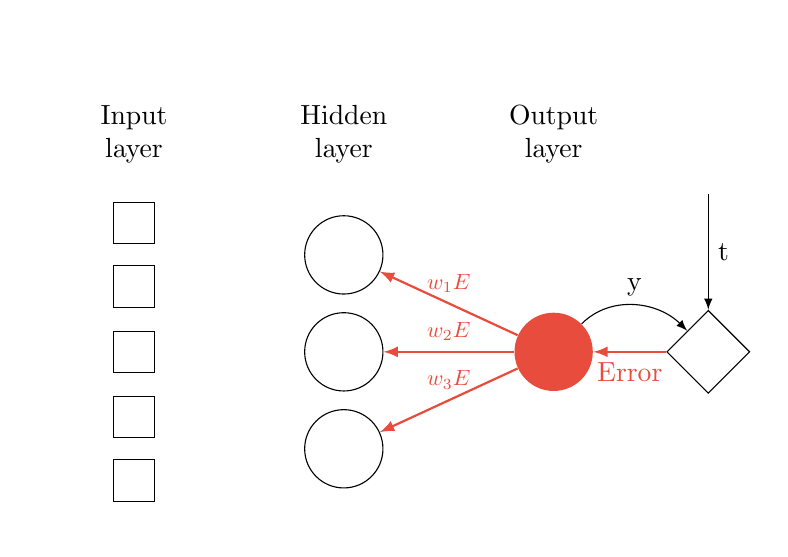
\begin{tikzpicture}[
  plain/.style={
    draw=none,
    fill=none,
  },
  input/.style={
    draw,
    rectangle,
    fill=none,
    minimum width=1.5em,
    minimum height=1.5em,
    inner sep=0pt,
  },
  error/.style={
    draw,
    diamond,
    fill=none,
    minimum width=3em,
    minimum height=3em,
    inner sep=0pt,
  },
  nerror/.style={
    draw=none,
    fill=reddish
  },
  net/.style={
    matrix of nodes,
    nodes={
      draw,
      circle,
      inner sep=10pt
    },
    nodes in empty cells,
    column sep=0.2cm,
    row sep=-17pt
  },
  >=latex
]

\matrix[net] (mat) {
  % Text row
  |[plain]| \parbox{1.3cm}{\centering Input\\layer} &
  |[plain]| \parbox{1.3cm}{\centering Hidden\\layer} &
  |[plain]| \parbox{1.3cm}{\centering Output\\layer} &
  |[plain]| \\
  % Nodes
  |[input]| & |[plain]| & |[plain]| & |[plain]|\\
  |[plain]| &           & |[plain]| & |[plain]|\\
  |[input]| & |[plain]| & |[plain]| & |[plain]|\\
  |[plain]| & |[plain]| & |[plain]| & |[plain]|\\
  |[input]| &           & |[nerror]| & |[error]|\\
  |[plain]| & |[plain]| & |[plain]| & |[plain]|\\
  |[input]| & |[plain]| & |[plain]| & |[plain]|\\
  |[plain]| &           & |[plain]| & |[plain]|\\
  |[input]| & |[plain]| & |[plain]| & |[plain]|\\
};

% Arrows 2
\draw[<-,reddish,thick] (mat-3-2) -- node[above=1pt,scale=0.8]{$w_1 E$} (mat-6-3);
\draw[<-,reddish,thick] (mat-6-2) -- node[above=1pt,scale=0.8]{$w_2 E$} (mat-6-3);
\draw[<-,reddish,thick] (mat-9-2) -- node[above=1pt,scale=0.8]{$w_3 E$} (mat-6-3);

\draw[->] (mat-6-3.north east) to [out=45,in=135] node[above]{y} (mat-6-4);
\draw[<-] (mat-6-4) to node[right] {t} +(0,2cm);
\draw[<-,reddish,thick] (mat-6-3) to node[below]{Error} (mat-6-4) ;

\end{tikzpicture}
\end{document}
